% !TEX root = ../thesis.tex
\chapter{Lit Review}
	\label{chap:lit_review}
	Education and the sharing of knowledge is a powerful tool. In fact, in our opinion the most important skill anyone can have. As a famous quote said, "give a man a fish, and he will starve, but teach him to fish, and he won't be hungry anymore". However, it wasn't until 1918 that education, as most people in England and Wales have experienced, started to come into effect \cite{education1918}.
	
	Education over the years was very much about just giving the knowledge to the students from the teacher. It wasn't until 1988, under the Education Reforms Act 1988, that assessments got introduced. The introduction was through the introduction of the national curriculum in England and Wales \cite{education1988}.
	
	As the curriculum got rolled out, statutory assessments got introduced to education between 1991 and 1995. Key Stage 1 first, followed by Key Stages 2 and 3, respectively \cite{hutchison1994reliable, dillon2011becoming}. Only for the core subjects of English, Mathematics and Science had the assessments first introduced. The first assessments in Key Stage 1 were a range of cross-curricular tasks to be delivered in the classroom, known as standardised assessment tasks - hence the common acronym 'SATs'. However, the complexity of the use of these meant more formal assessments quickly replaced them \cite{hutchison1994reliable, dillon2011becoming}. The assessments in Key Stages 2 and 3 got developed using more traditional tests.
	
	To allow teachers to judge students' attainment, taking tests became the main assessment form in key stage 3. While assessments were the main form, educators were also able to assess their students with other means against the targets set for attainment within the national curriculum \cite{dillon2011becoming}. The teacher and assessment outcomes got used on a scale with key learning milestones expected at different ages. A key stage level indicated the result for the students progress. The model was used throughout the next few years until 2005 when the role of tests in KS1 got downgraded to just being an internal support tool to teachers, and in then 2008, the government decided to remove tests in KS3 \cite{dillon2011becoming}.
	
	This model continued, with minor adjustments to reflect the changing content of the National Curriculum, up to 2004. From 2005, the role of the tests got downplayed at Key Stage 1, with tests being used only internally to support teacher assessment judgements \cite{bbc_no_tests}. Further changes came in 2008 when the government announced that testing in Key Stage 3 was to get scrapped altogether \cite{bbc_tests_scrapped}.
	
	However, with a change of government party, the Conservative party taking power from the Labour party brought about new changes to how education's focuses and pedagogy methods would get conducted. In 2014 the system of attainment levels was removed, creating the educational shift of "Assessing without level" \cite{ass_without_lvls}. However, within schools, it was being referred to as 'life after levels'. Especially by our educational colleges and us at the time. Which was the follow up to the changes in the national curriculum in 2013 \cite{ass_without_lvls}. The changes within the national curriculum brought a greater focus on more traditional style GCSE academic subjects while reducing the focus on perceived technical labour style jobs. The new curriculum direction created more emphasis on the final exam outcomes at the stages of GCSE and A-Level.
	
	\section{The Purpose of Assessment, Marking and Feedback in Education}
	As we have established, assessments became a staple of the UK educational system in 1988. While the term assessments are not usually defined, the word 'assess' is typically associated with measuring, determining, evaluating, and judging \cite{wellington2007secondary}.
	
	While there can be multiple reasons why educators assess students, assessments aim to serve a purpose to both the teacher and the student in the process. These include: giving feedback to teachers and learners; providing motivation and encouragement; to boost the self-esteem of the pupils; a basis for communication; a method to evaluate a lesson/training method/scheme of work/ curriculum; to entertain \cite{wellington2007secondary}. Additionally, the assessment also creates other opportunities to rank students; a method to select and filter students, allocate students a particular pathway or educational direction, or as a way to discriminate or choose between students for a given set reason \cite{wellington2007secondary}.
	
	\subsection{Traditional Methods of Assessment and Feedback} % Should these be subsections?
	There are four main categories of assessment. These are diagnostic, formative, summative, and national assessments \cite{wellington2007secondary, dillon2011becoming}. However, it is essential to note that national assessments do not get used within everyday aspects of teaching and learning. This term is the name given to the critical exams like SATS, GCSE and ALevel exams taken nationally. Therefore we will focus on the other three main ones.
	
	Diagnostic assessment is what gets referred to as pre-testing \cite{wellington2007secondary}. Educators use this technique to get a base level of knowledge of the students they have inherited. This method is good for showing the progress of attainment over time by having an initial base test. Teachers can then show how well the students have progressed over time with their improvements over the term. This base assessment also provides the teacher with crucial information - the current ability of every student's knowledge. Through knowing this current level of knowledge, teachers can adapt the coming lessons and provide suitable differentiation and scaffolding within the lessons to allow each student to succeed as much as possible. However, we also experienced, within our time as an educator, the technique getting used to create baseline narratives. Teachers were using them to show that the student's knowledge wasn't at the expected level when inherited by the teacher at meetings or performance management reviews. Therefore, being used as a counter-act measure tool by the teacher, if they find themselves being accused of letting the students' performance slip, by trying to counter-act by implying the students were not at the required level in the first place.
	
	The second method, formative assessment, is also known as 'assessment for learning (AFL)' \cite{wellington2007secondary, dillon2011becoming}. This method has become one of the main tools for a teacher in terms of assessment and feedback. AFL allows the educator to assess the students' understanding of a topic on the fly during a lesson without a summative assessment. As a result, allowing the teacher to spend more or less time if the students do or don't get the topic, even if they planned more or less time for that topic. Therefore, ensuring that the teaching is not getting carried out for teaching sake. Thus, the emphasis is less on measurements and more on actual learning. AFL can involve using several techniques: teacher assessment - through in-class questions, marking books; to the students assessing their work called self-assessment, or peer assessment - where the students evaluate each other's work \cite{wellington2007secondary}.
	
	The third method is a summative assessment, also known as 'assessment of learning (AOL) \cite{wellington2007secondary}. This type of assessment happens at the end of a teaching unit or topic. It gets used to gain insights into what the students have learnt within the subject covered or the course. Its purpose is to give a student a mark, grade or ranking. Usually, this is the grade that is mainly focused on, as it is the metric that will impact the school the most in terms of league performance tables regarding GCSE and A-level results. From our experience, summative assessments are carried out regularly within schools. This assessment method tends to get used to getting a snapshot of the students of whit if a moment like, if they were to take the test now, what would they get? By seeing the results, educators can see if students need to attend intervention or if they are performing as expected or even better. With so much riding on these results, for schools and teachers performance management reviews, a lot of emphasis on put into trying to predict the final results for students. We have seen it put a lot of pressure on the teachers and the students and ultimately creates a very stressful environment, which is not the best environment for learning.
	
	
	
	
	\subsection{Why Traditional Traditional Marking and Feedback Methods are Effective}
	
	
	\subsection{The Negative Aspects of Traditional Marking and Feedback Methods}
	
	\section{Comparative Judgement}
	
	
	\subsection{What is Comparative Judgement} 
		Comparative judgement is a mathematical way to determine which observation item is better than the other item also being observed compared to each other. This method was first proposed in 1927 by Louis Leon Thurstone, a psychologist, under the term "the law of comparative judgement" \cite{thurstone1927psychophysical, thurstone1927law}. In modern-day terminology, it gets more aptly described as a model used to obtain measurements from any pairwise comparison process. Examples of such methods are comparing the perceived intensity of physical stimuli, such as the weights of objects, and comparing the extremity of an attitude expressed within statements, such as statements about capital punishment. The measurements represent how we perceive things rather than being measurements of actual physical properties. This kind of measurement is the focus of psychometrics and psychophysics. <wikipedia>
		
		In more technical terms, the law of comparative judgment is a mathematical representation of a discriminal process. This process involves a comparison between pairs of a collection of entities concerning multiple magnitudes of attributes. The model's theoretical basis is closely related to item response theory and the theory underlying the Rasch model. These methods are used in psychology and education to analyse data from questionnaires and tests.
		<wikipedia>
		
		While comparative judgement is a technique that has been around for almost 100 years, it wasn't until the early nineties that this technique got proposed for use within an educational setting. This first proposal was by Politt and Murry \cite{pollitt1996raters}, who conducted a study where they tested candidates on their English proficiency within Cambridge's CPE speaking exam. The judges watched 2-minute videos and judged which one out of a pair of videos they deemed better at the requested task in the exam. However, before this, in the ninety seventies and eighties, comparative judgement was presented as a more theoretical basis for educational assessments \cite{andrich1978rating}. 
		
		With the momentum of his findings, Politt then presented comparative judgement as a tool for exam boards to use to be able to compare the standards of A-Levels from the different exam boards, replacing the direct judgement of a script that was at the time currently being used \cite{newton2007paired}. In his papers titled, "Let's Stop Marking Exams" \cite{stop_marking_pollitt}, he presents a valid argument for using comparative judgement, with the advantages it brings over some traditional types of marking.
		
		Politt, in 2010, also presented a paper at the Association for Educational Assessment – Europe. It was about How to Assess Writing Reliably and Validly. Politt presented evidence of the extraordinarily high reliability achieved with Comparative Judgement in assessing primary school pupils' skill in first-language English writing \cite{pollitt2009abolishing}.
		
	\subsection{The Logic Behind Comparative Judgement and What it Aims to Do} % Should these be subsections?
		How comparative judgement works is to present two options to a marker. The marker then gets asked to pick which one of the two options they think is the better one. The marker will get presented with all possible combinations available, each time picking which one they think is the better one out of the two. An outputted score is then presented based on the method used. The original method, the Law of Comparative Judgement (LCJ), follows the formula:
		
		\begin{figure}[h]
			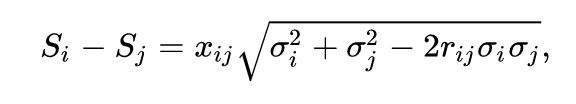
\includegraphics[width=8cm]{graphics/LCJ_formula.png}
			\caption{}
			\centering
		\end{figure}
	
		 $S_{i}$ is the psychological scale value of stimuli $i$
		%{\displaystyle x_{ij}} is the sigma corresponding with the proportion of occasions on which the magnitude of stimulus i is judged to exceed the magnitude of stimulus j
		%{\displaystyle \sigma _{i}} is the discriminal dispersion of a stimulus {\displaystyle R_{i}}
		%{\displaystyle r_{ij}} is the correlation between the discriminal deviations of stimuli i and j
		%The discriminal dispersion of a stimulus i is the dispersion of fluctuations of the discriminal process for a uniform repeated stimulus, denoted {\displaystyle R_{i}}, where {\displaystyle S_{i}} represents the mode of such values. Thurstone (1959, p. 20) used the term discriminal process to refer to the "psychological values of psychophysics"; that is, the values on a psychological continuum associated with a given stimulus.
		
		However, an alternative version derived from Louis Leon Thurstone, referred to as the "Pairwise Comparison" \cite{thurstone1927law}, will provide an output based on the difference between the quality values is equal to the log of the odds in respect to object-A will be object-B. This formula gets represented as: 
		$\displaystyle \mathrm {log\;odds} (A\ {\text{beats}}\ B\mid v_{a},v_{b})=v_{a}-v_{b} $.
		
		$\Pr\{X_{ji}=1\}={\frac {e^{{\delta _{j}}-{\delta _{i}}}}{1+e^{{\delta _{j}}-{\delta _{i}}}}}=\sigma (\delta _{j}-\delta _{i})$
		
		 .
		%\displaystyle \mathrm {log\;odds} (A\ {\text{beats}}\ B\mid v_{a},v_{b})=v_{a}-v_{b}}		


	\subsection{How effective is Comparative Judgement at Providing Feedback?} % Should these be subsections?
		
		

	\section{Related Work}
		\label{sec:google_fu}



	\subsection{Subsection all similar work}
		\label{sec:resources_bibtex}
	


	\subsection{Comparison of similar work}
